\chapter{Results and Discussion}\label{ch:results_discussion}
This chapter presents the results of our experiments as described in Chapter~\ref{ch:methods}. 

\section{Results}\label{results}
In this section we present the results of our experiments, beginning with genome size. 

It is of minor note that in many of the figures, a rolling window was used to smooth the values, resulting in many of the plots only showing data starting after a few thousand generations (often 10,000). The data are complete, however. 

\subsection{Genome Size}
In this section we will examine the results of the different conditions, focusing on which, if any, lead to a reduced genome. Figure~%TODO add figure showing genome size
presents the main findings regarding genome size. In the Figure, the blue line %TODO make sure the line is actually the blue one
represents the control condition and the other colors show the changed conditions: mutation up/down, selection up/down, and population up/down. As can be seen from the figure, 
\begin{figure}[H]
	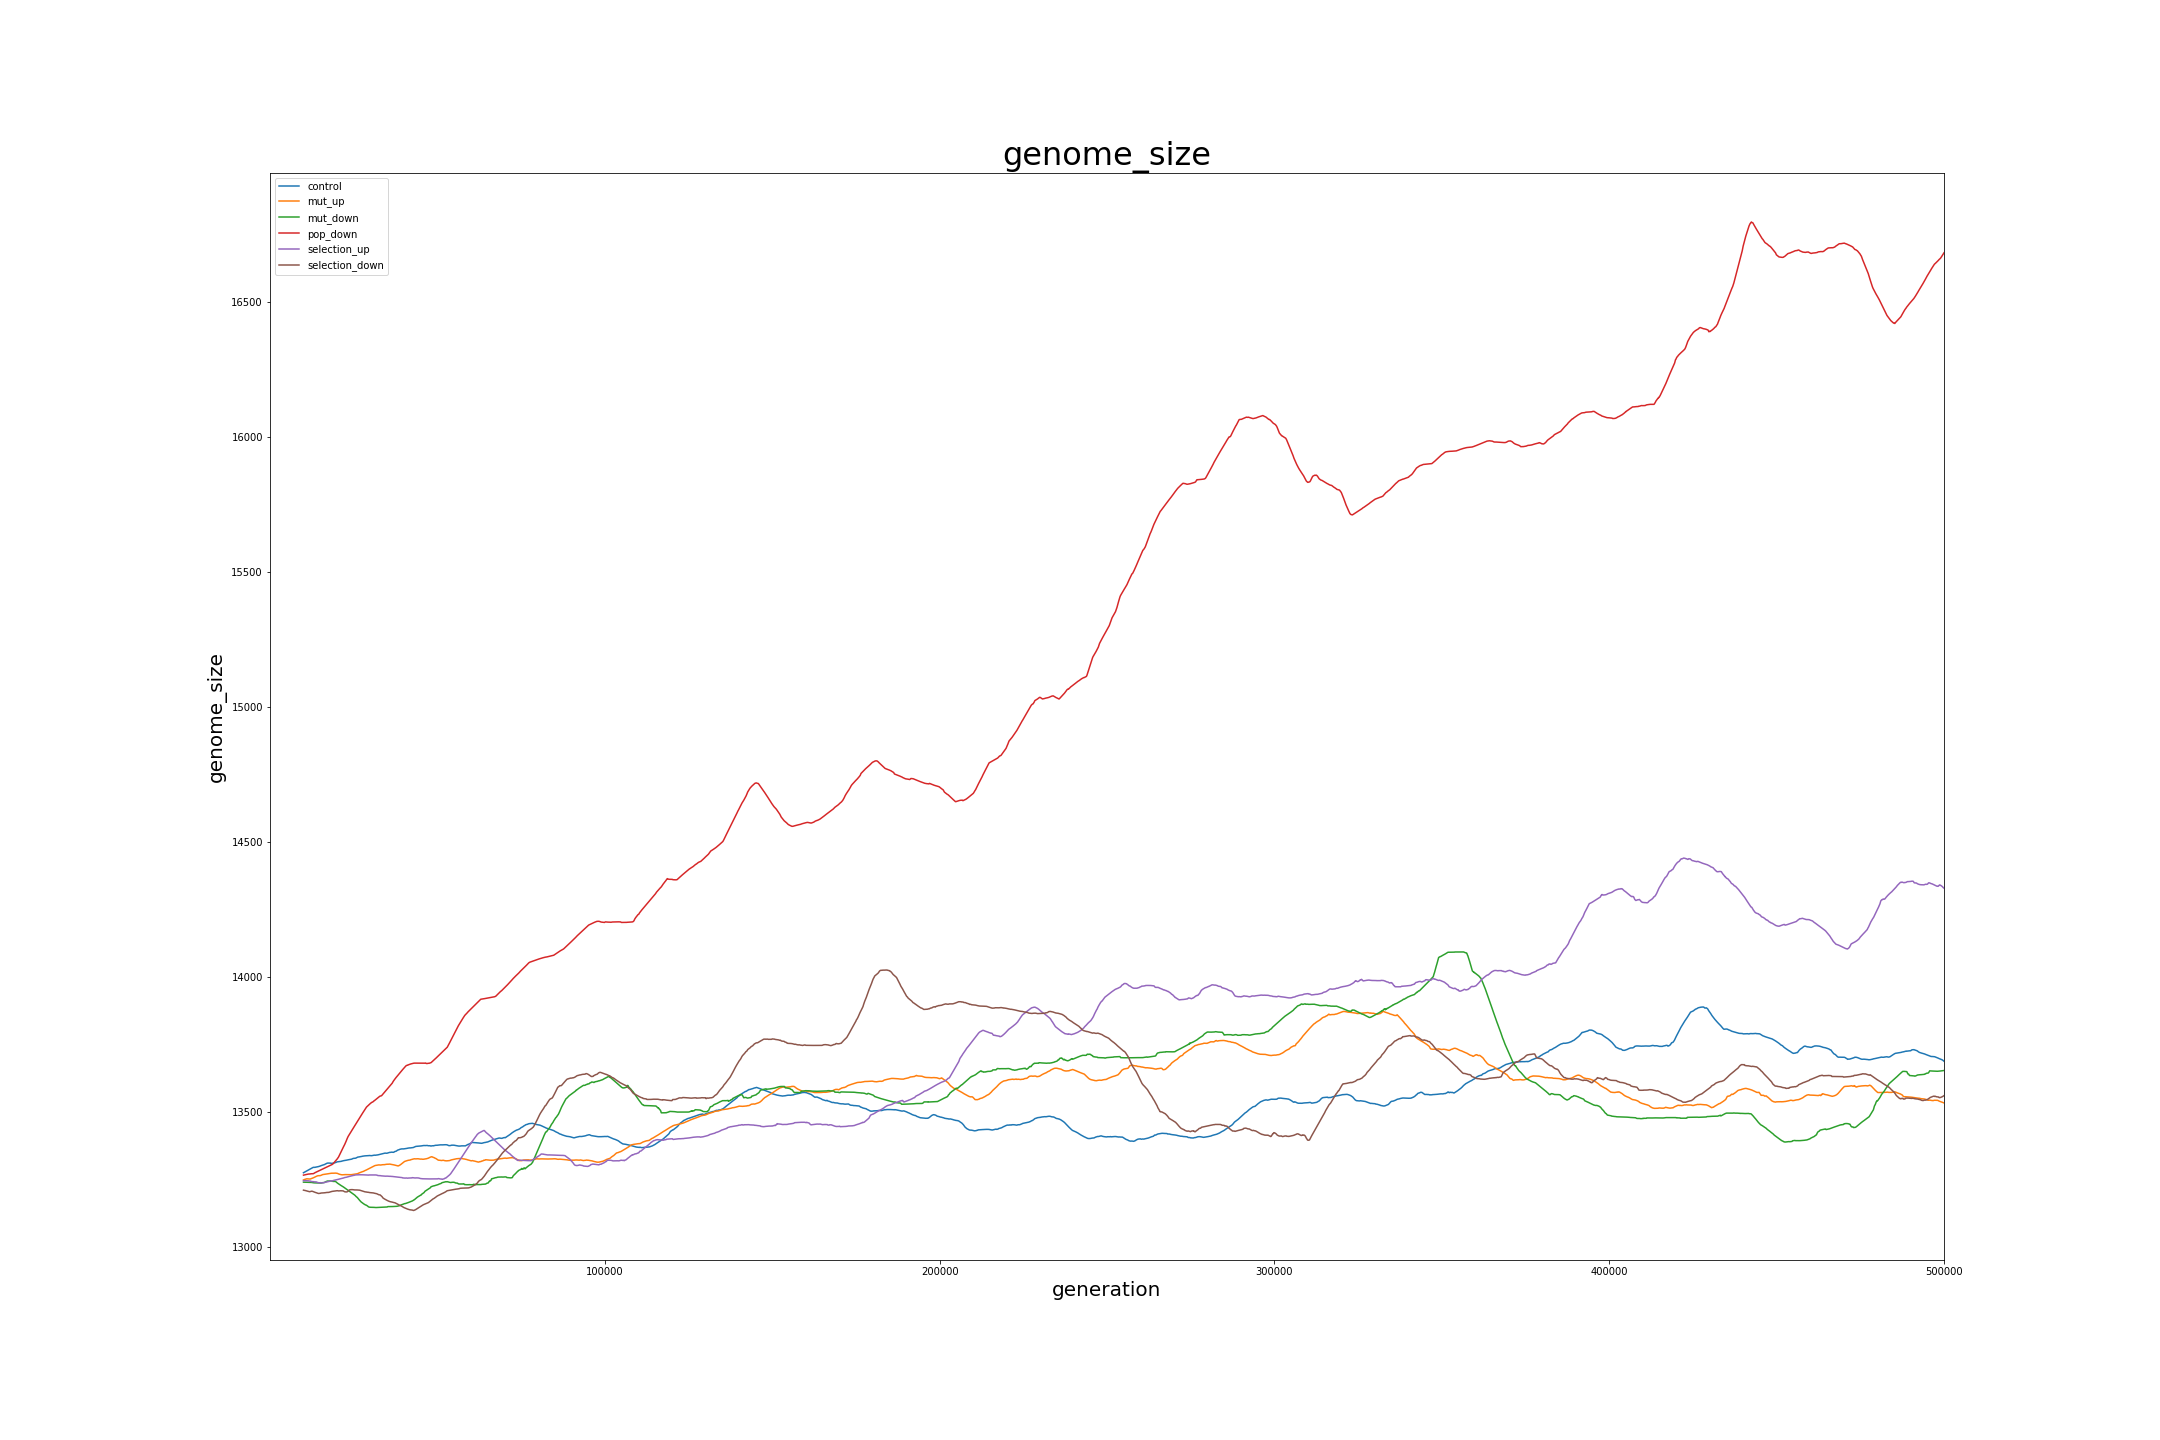
\includegraphics[width=\linewidth]{stat_fitness_mean_genome_size}
	\centering
	\caption[Genome size]{Genome size in number of bases of all conditions. Average taken across all five seeds for each condition.}
	\label{fig:genome_size}
\end{figure}
The most conspicuous observation is that none of the conditions resulted in a reduced genome size, and in fact the \textit{population down} condition had a runaway increase in the number of bases, reaching as high as 16,500 bases, a 25\% increase over the original wild type's roughly 13,200. Surprisingly, even after 500,000 generations it seems that the upper limit may still not have been reached. 

The next obvious observation is that of the remaining conditions, only the \textit{selection up} condition seems to have made much of a significant change with its 11\% increase. All of the remaining conditions had a mild increase in genome size. 

Also noteworthy is that the mutation down condition appears to have had a steady increase in the number of base pairs until a maximum of just over 14,000 around generation 350,000 before having a fairly sharp decline back to nearly the original size. 

\subsection{Metabolic Error}
\begin{figure}[H]
	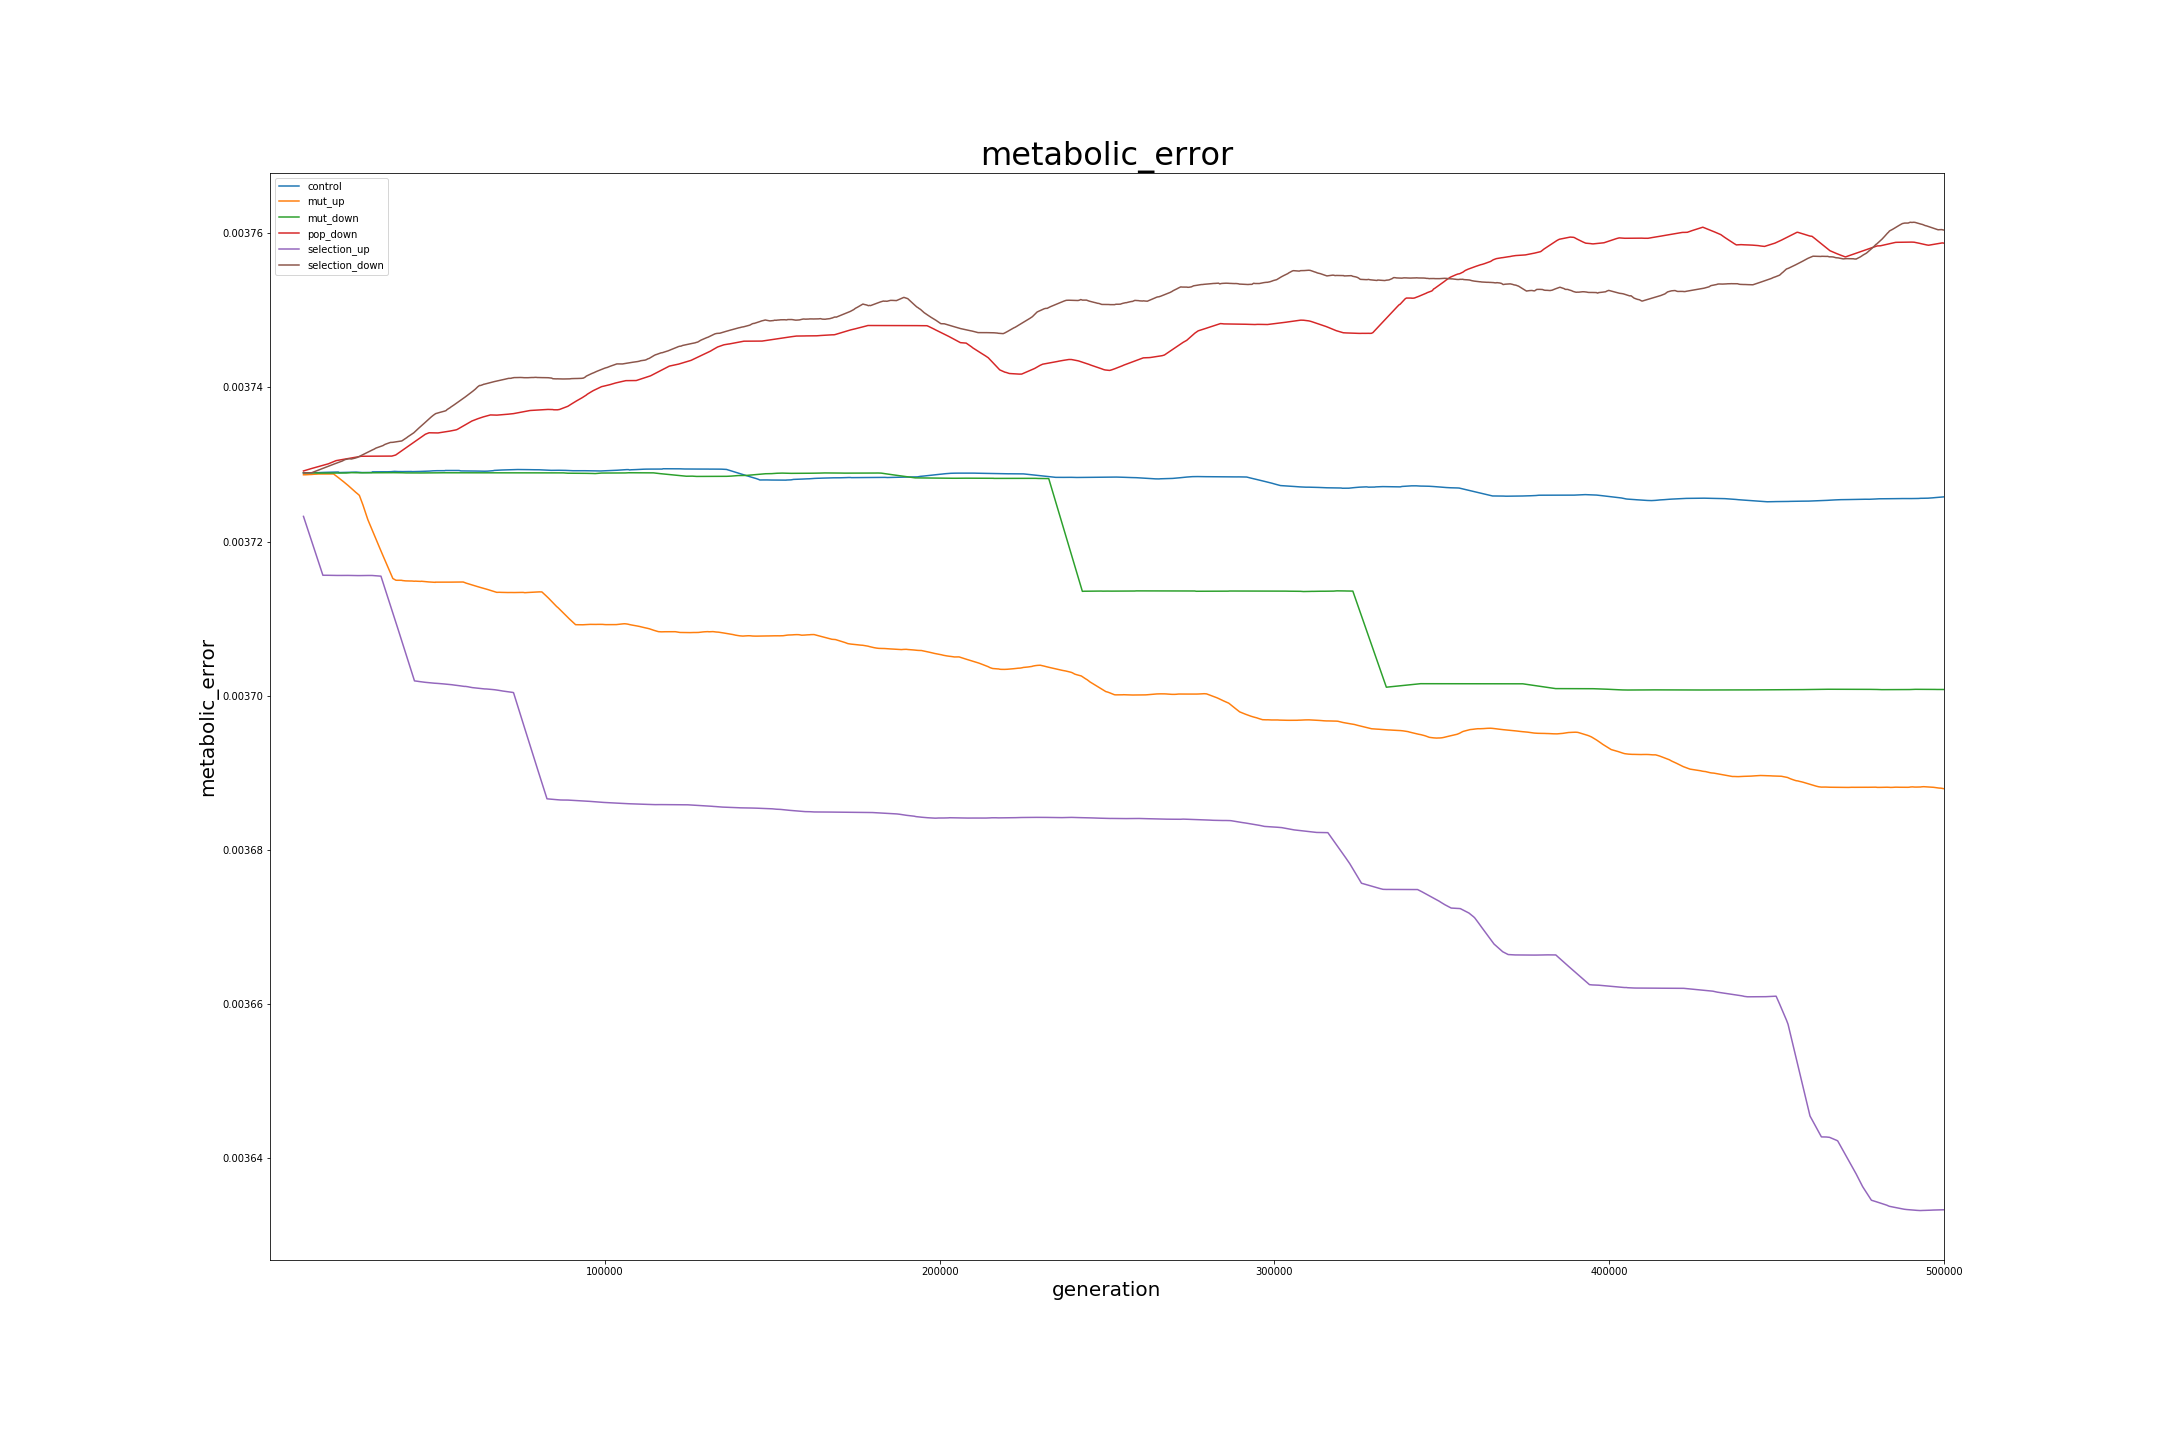
\includegraphics[width=\linewidth]{stat_fitness_mean_metabolic_error}
	\caption[Metabolic error]{Plot of the metabolic error over time for all conditions, average of all seeds}
	\label{fig:mean_metabolic_error}
\end{figure}
\subsection{Genome Structure}
In this section we examine the effects of the differing conditions on the structure of the genome as measured by the criteria in Tables~\ref{table:aevol_stats_genes_and_bp} and~\ref{table:aevol_stats_fitness_and_mutation}. 
\subsubsection{Non-coding DNA}
One important factor in genome structure is the amount of non-coding DNA, i.e. the number of bases which are part of a genome but which do not encode protein sequences. In the case of aevol, this means 
\begin{figure}[H]
	\centering
	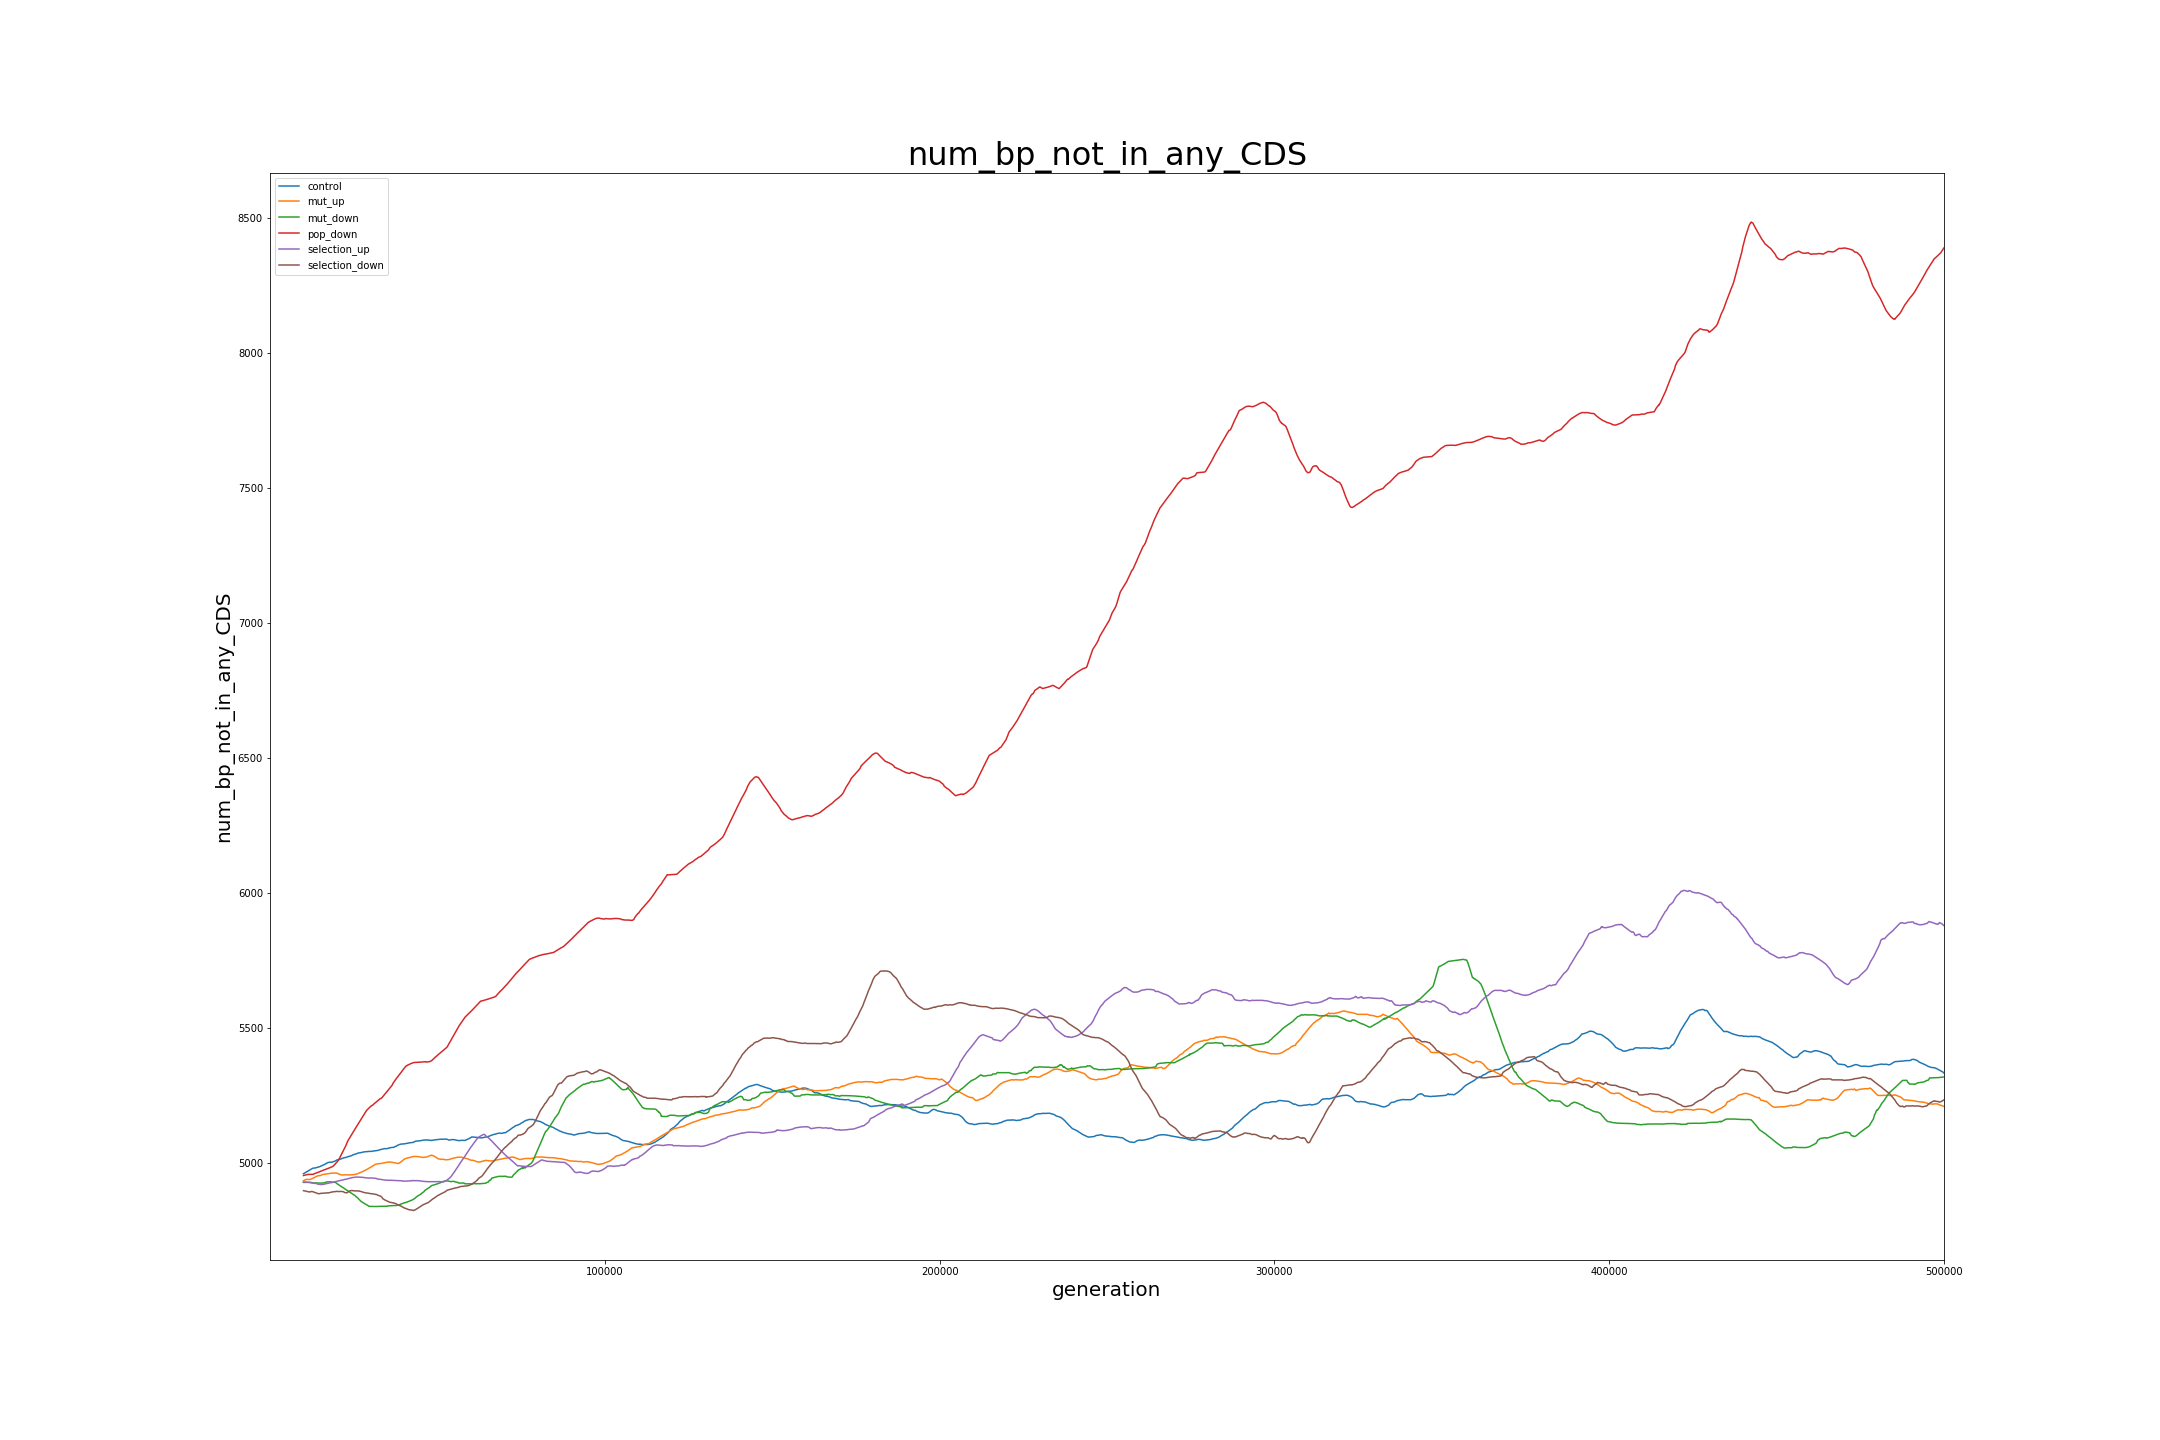
\includegraphics[width=\linewidth]{stat_bp_mean_num_bp_not_in_any_CDS}
	\caption[Non-coding DNA]{Plot of non-coding DNA over time for all conditions, average of all seeds.}
	\label{fig:mean_non-coding_DNA}
\end{figure}

\subsubsection{Number of Genes}
\begin{figure}[H]
	\centering
	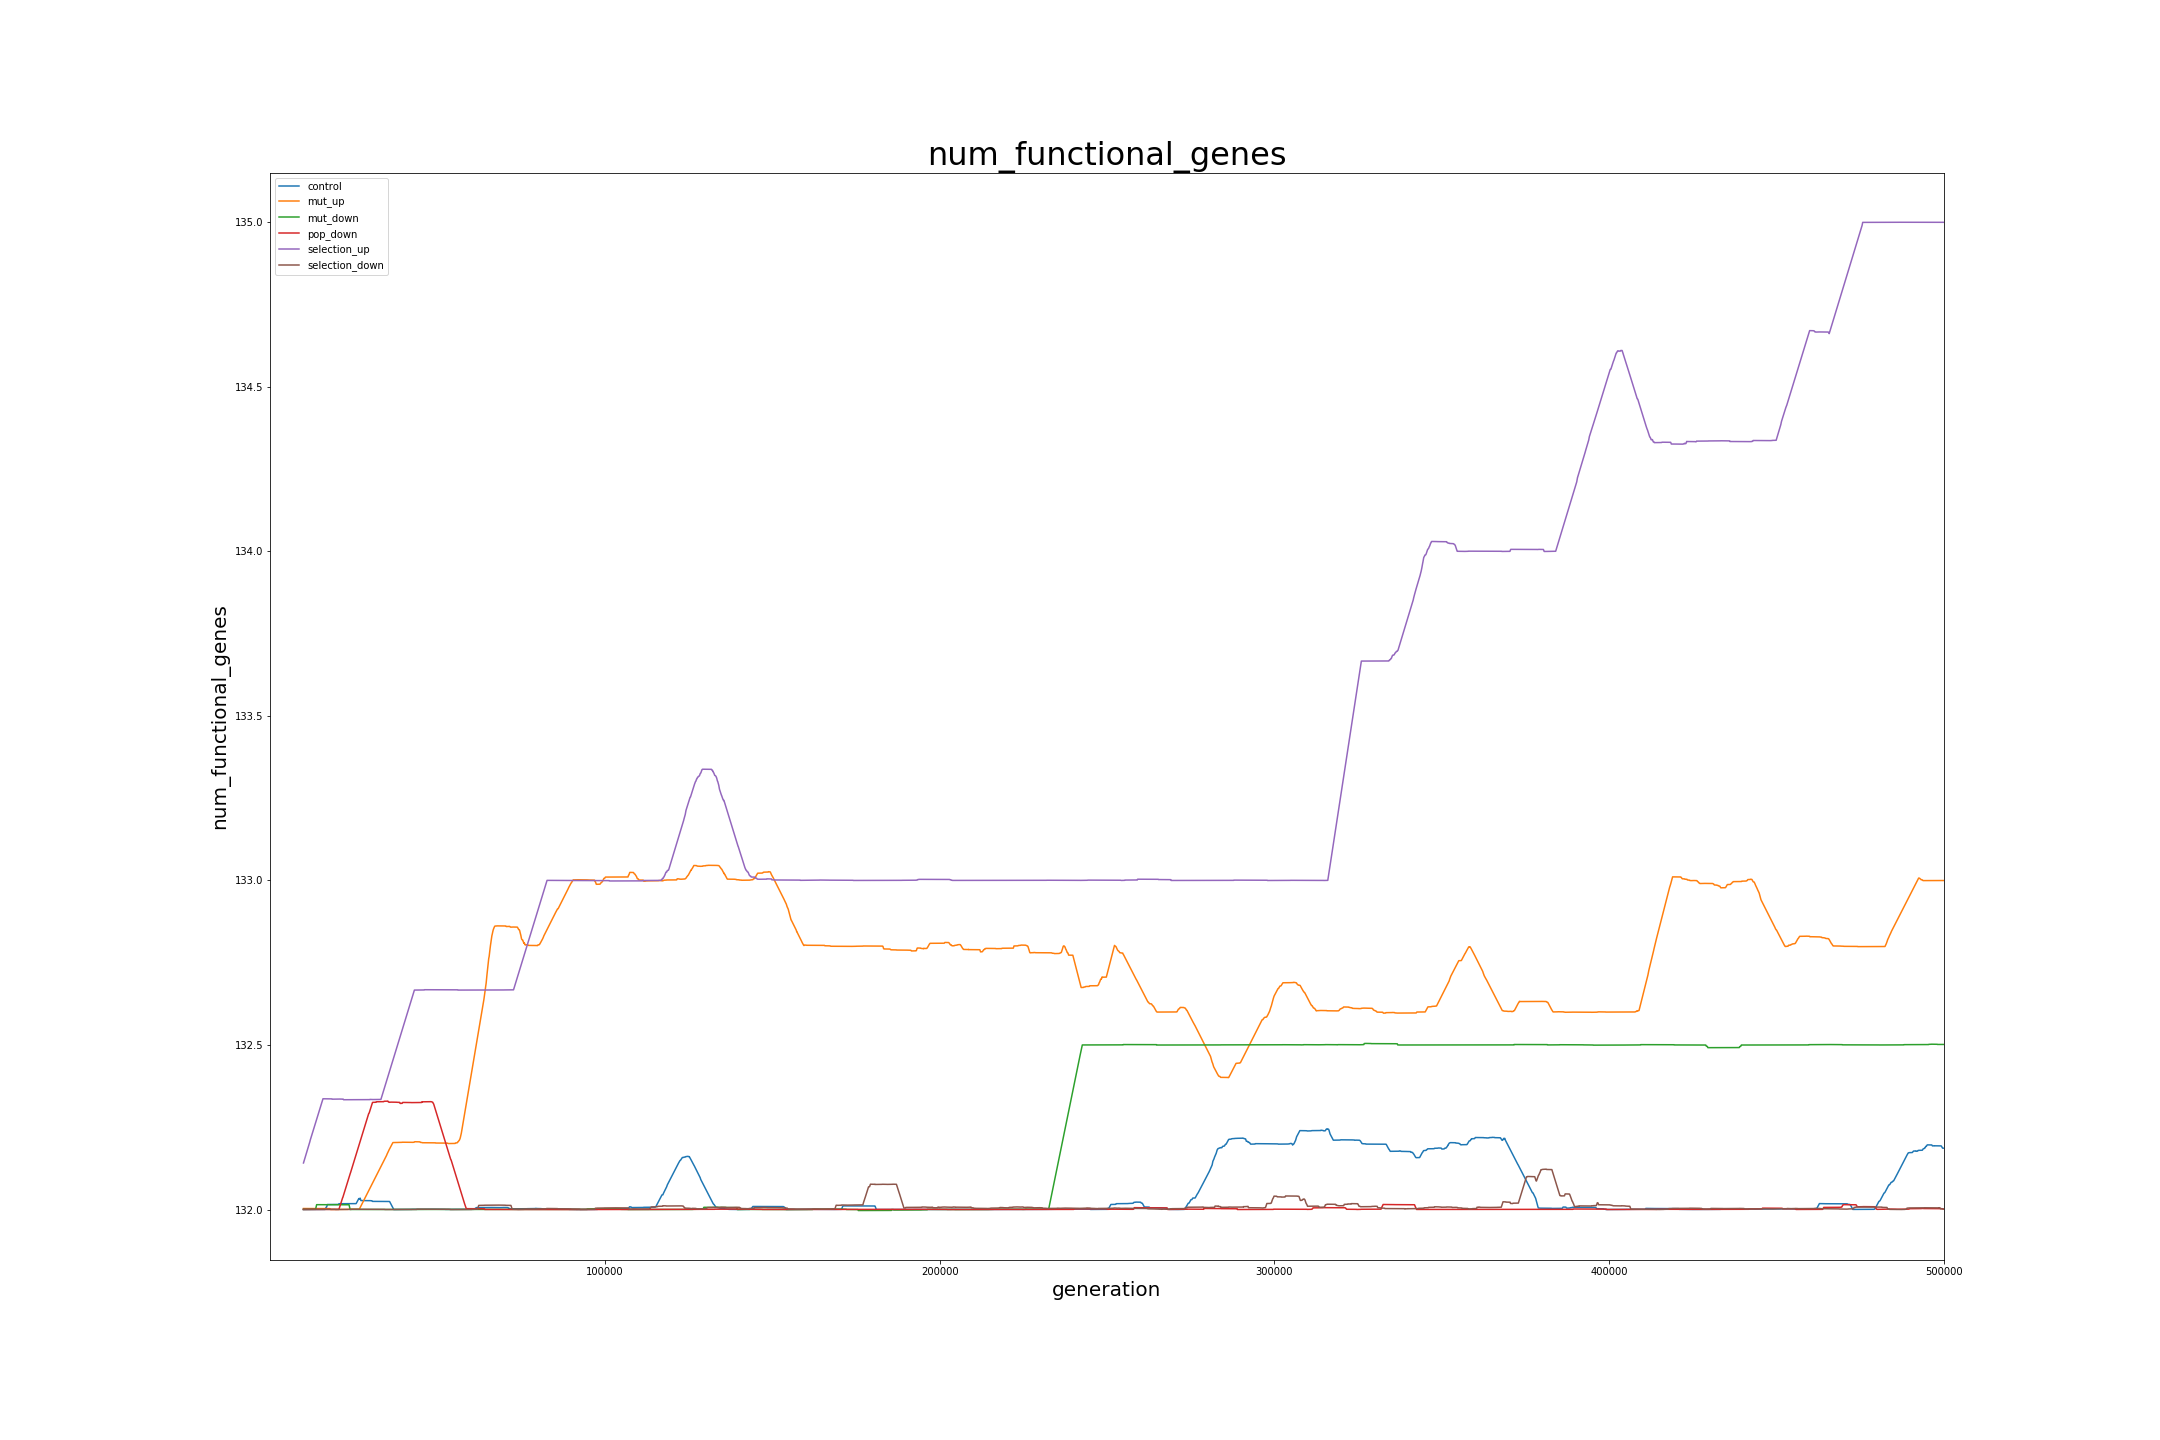
\includegraphics[width=\linewidth]{stat_genes_mean_num_functional_genes}
	\caption[Mean number of functional genes]{Plot showing the mean number of functional genes over time across all seeds.}
	\label{fig:mean_num_functional_genes}
\end{figure}
Interesting that so many of the lines are so flat and the mutation up line is so wiggly. Clearly the increased mutation rate was creating and destroying genes, whereas in the other cases it was a pretty even rate. 
\subsubsection{Average Size of Functional Genes}
\begin{figure}[H]
	\centering
	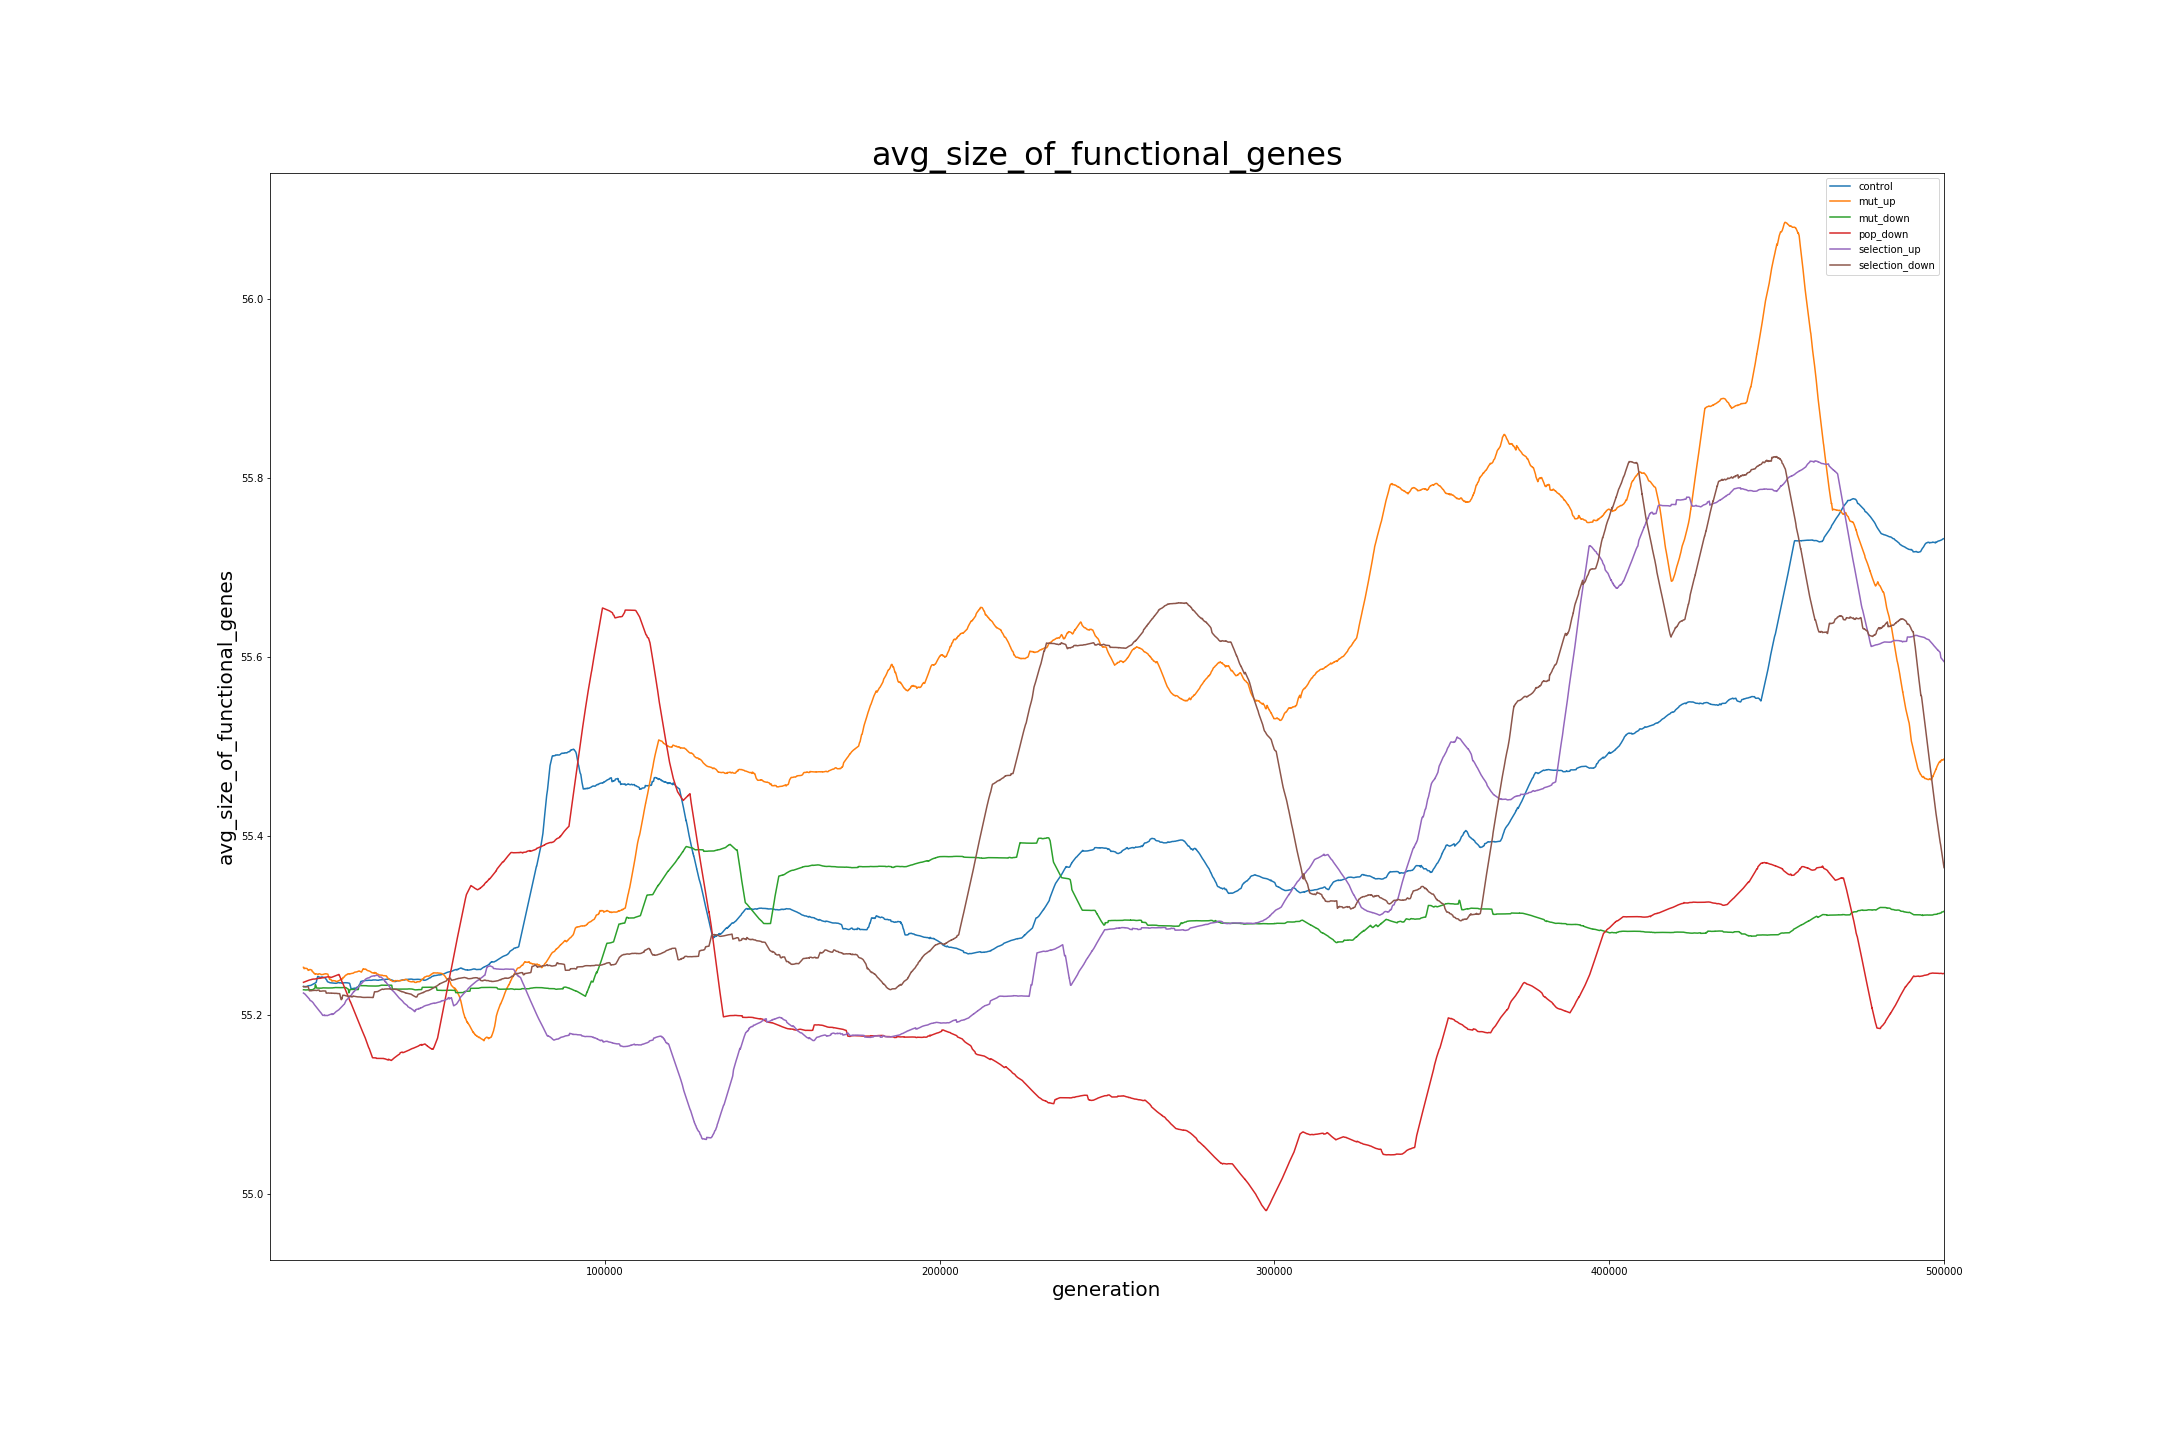
\includegraphics[width=\linewidth]{stat_genes_mean_avg_size_of_functional_genes}
	\caption[Average size of functional genes]{Plot showing the average size of functional genes over time for all seeds.}
	\label{fig:mean_functional_gene_size}
\end{figure}

\subsection{Evolvability}

\subsection{Robustness}
Recall that robustness is measured by the fraction of neutral mutants of an individual. In the following figure, we see a bar plot showing the spread of neutral mutants for the best individual for the control condition as well as the six variations. 

%TODO update graphic with more conditions once experiments are completed
\begin{figure}[H]
	\centering
	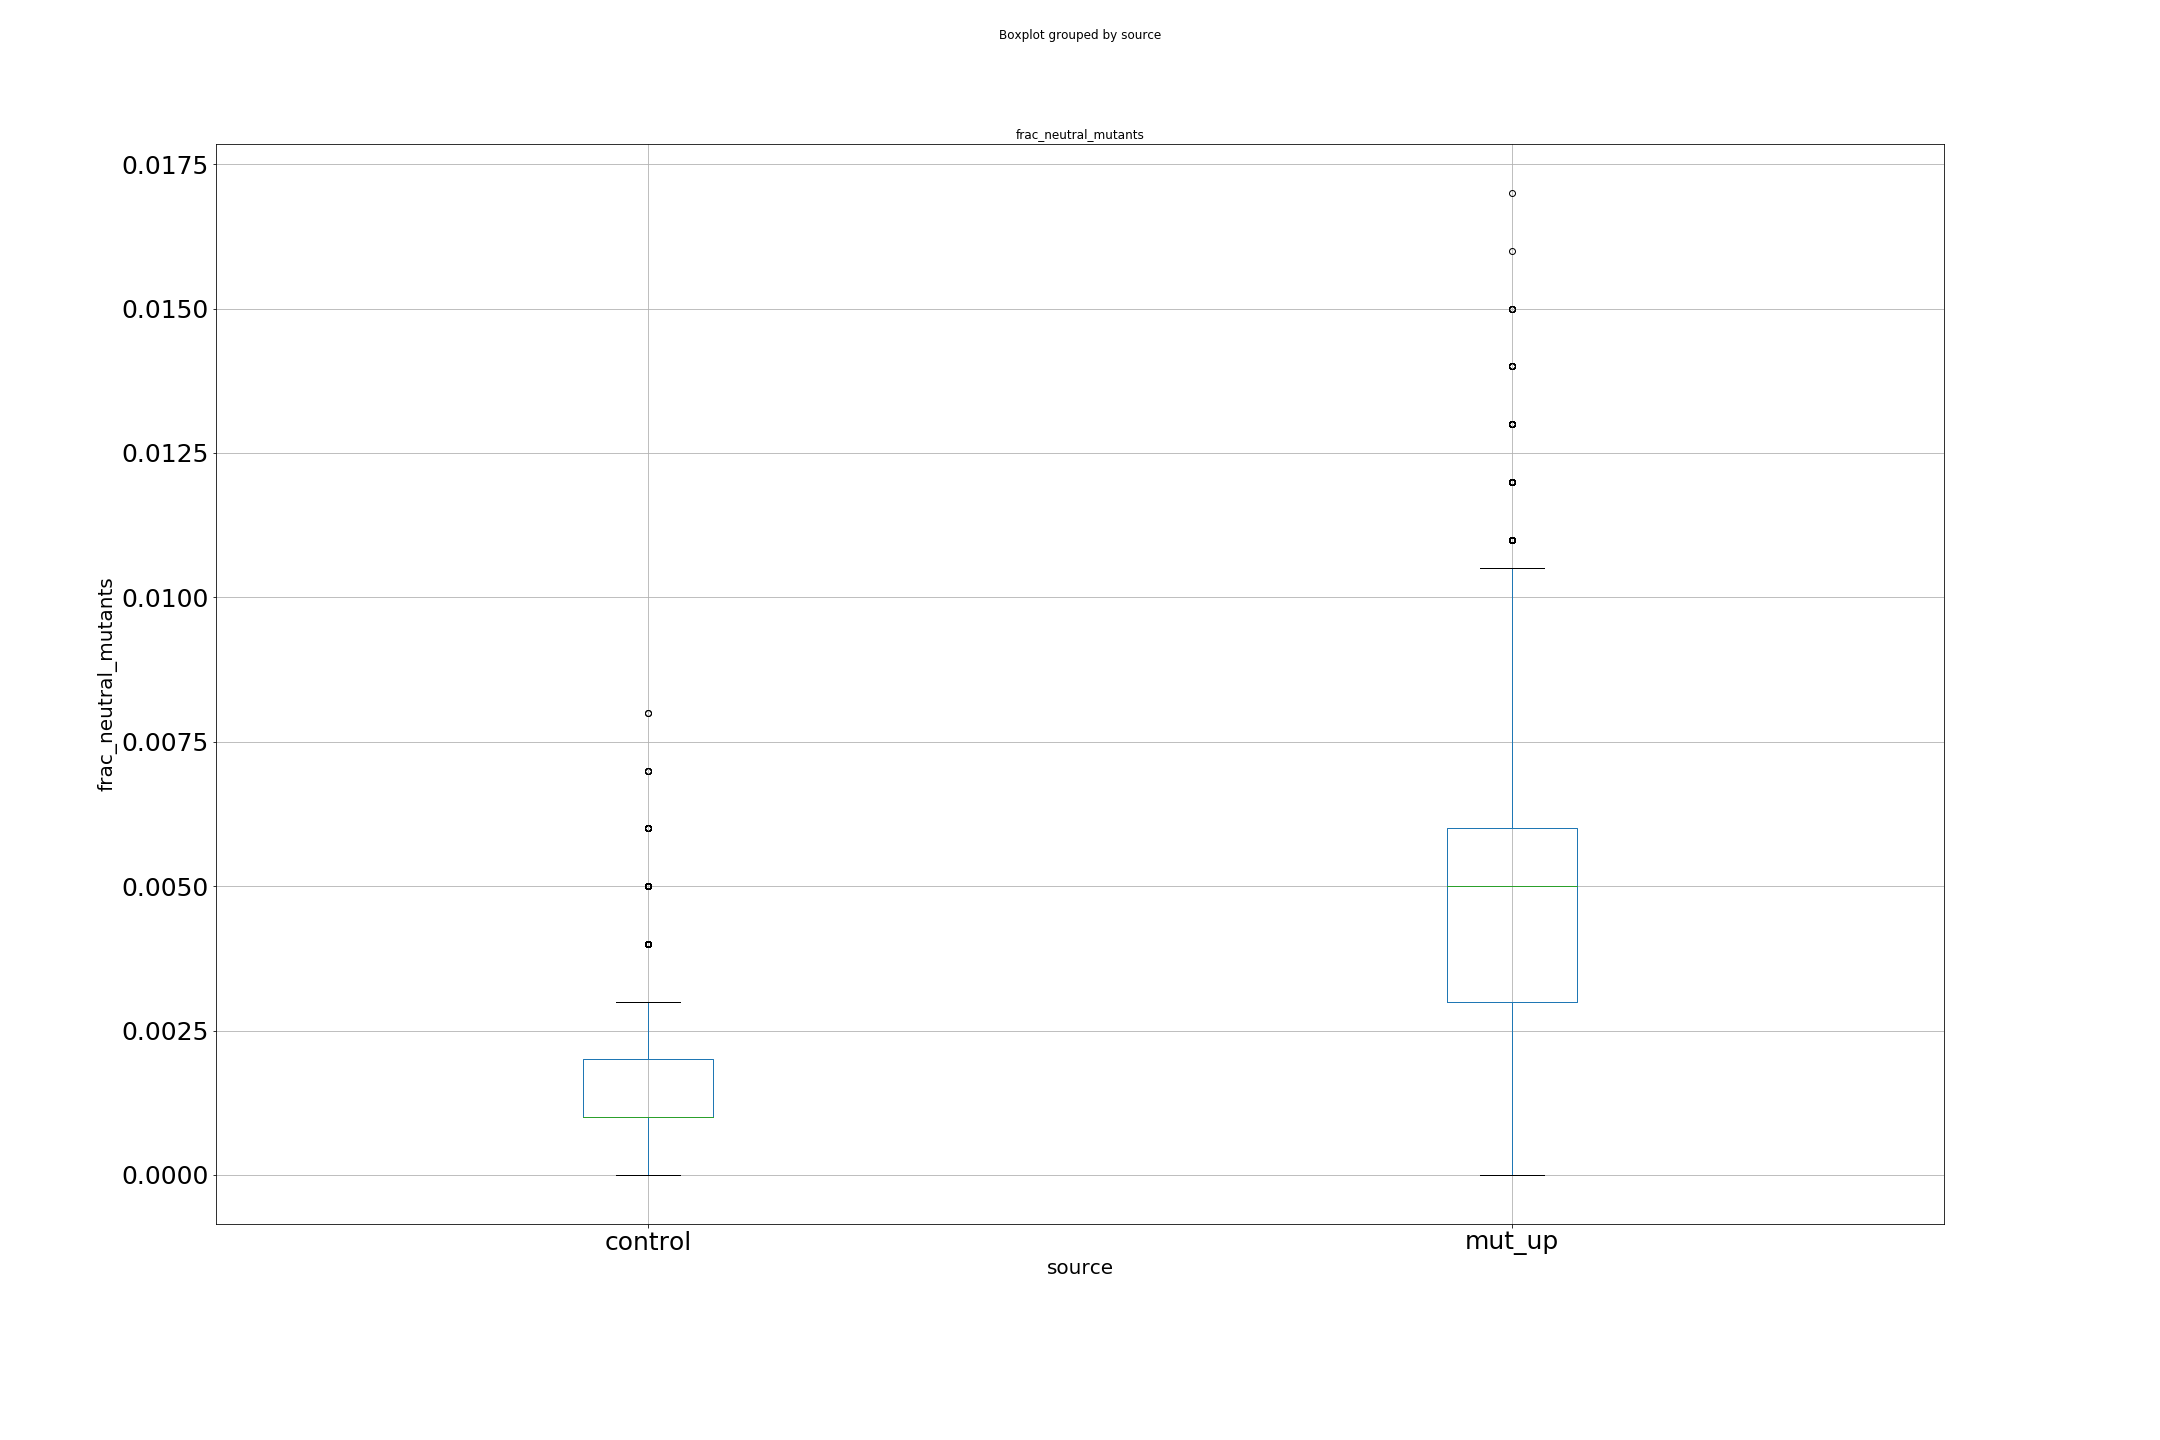
\includegraphics[width=\linewidth]{stat_robustness_mean_frac_neutral_mutants}
	\caption[Robustness bar graph]{Bar graph showing the spread of neutral mutants for the best individual at generation 500,000, all conditions.}
	\label{fig:mean_robustness_all_conditions}
\end{figure}

\section{Discussion}\label{discussion}

\subsection{Relation to Real-World Biological Entities}
%TODO Complete this section
\subsection{Limitations of Results}\label{limitations}
One limitation to consider is that only one parameter varied per condition. It may be possible that it is only under a combination of conditions (e.g. low selection \textit{and} high mutation rates) does reductive evolution occur. 

Another limitation is that the environments did not vary in our experiments. This could potentially have a large effect on robustness and evolvability, which are strong influencers of reductive evolution. 

Aevol as a modeling software is limited in that it relies, like all models, on several simplifications. The population sizes tested here, even in the population up condition, are still much smaller than would be found in real world populations. 